Накопление спектра производим в течение 600 секунд. Спектры представим на рис.
1-6. Проведём измерение фона (см. рис. 7) и убедимся, что интенсивность его
спектра много меньше интенсивности спектра исследуемых образцов; также в спектре
фона нет пиков.

\begin{figure}
\begin{center}
  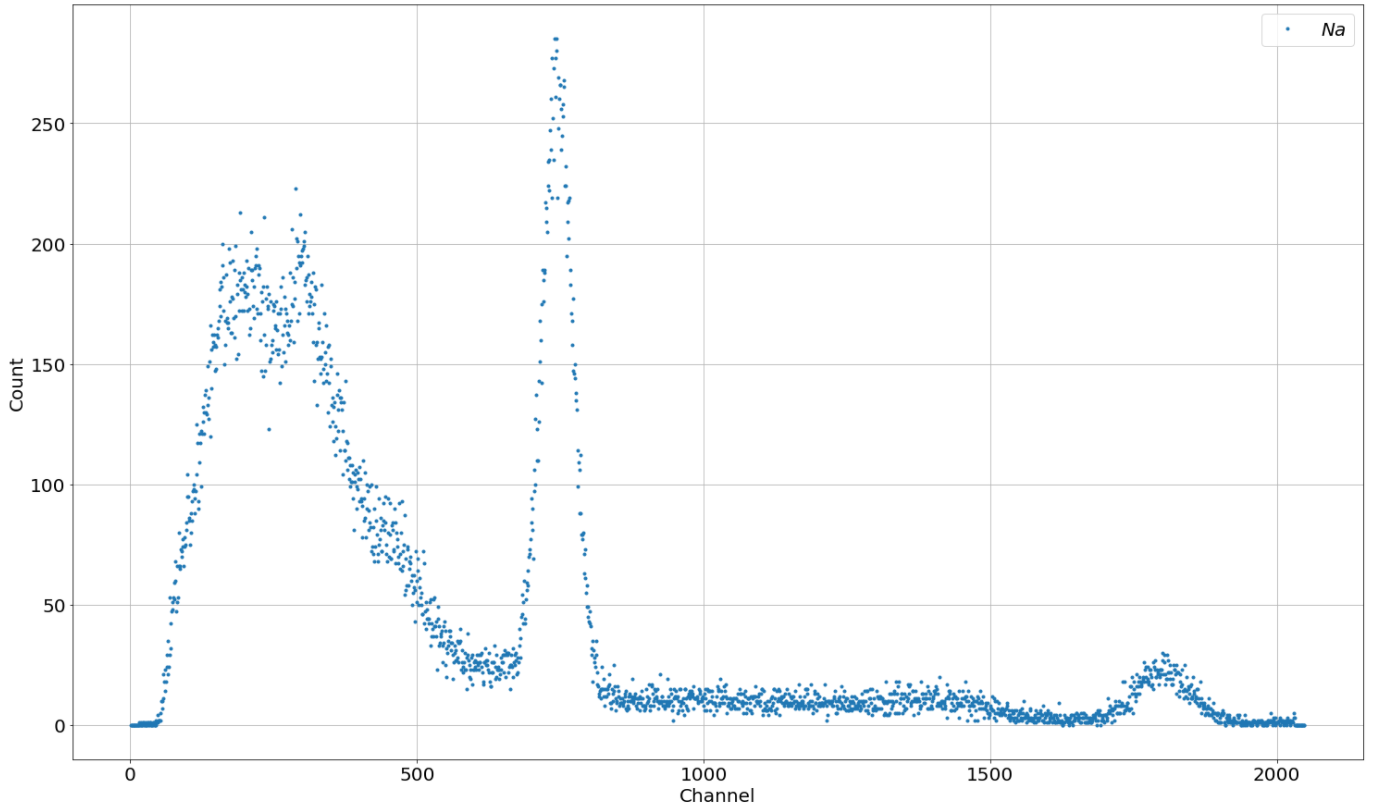
\includegraphics[width=0.8\linewidth]{Na.png}
  \caption{Спектр ${}^{22}{\text{Na}}$}
  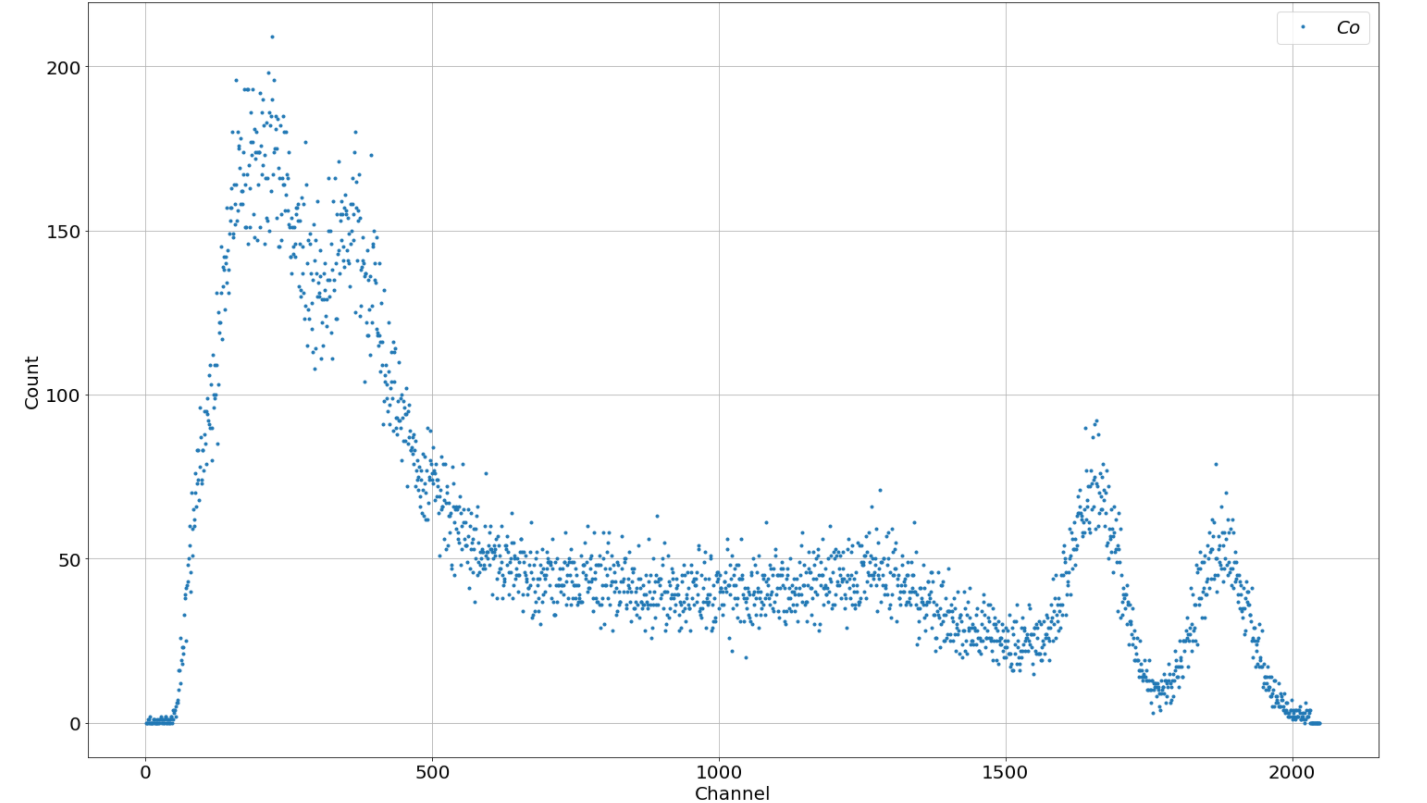
\includegraphics[width=0.8\linewidth]{Co.png}
  \caption{Спектр ${}^{60}{\text{Co}}$}
\end{center}
\end{figure}

\begin{figure}
\begin{center}
  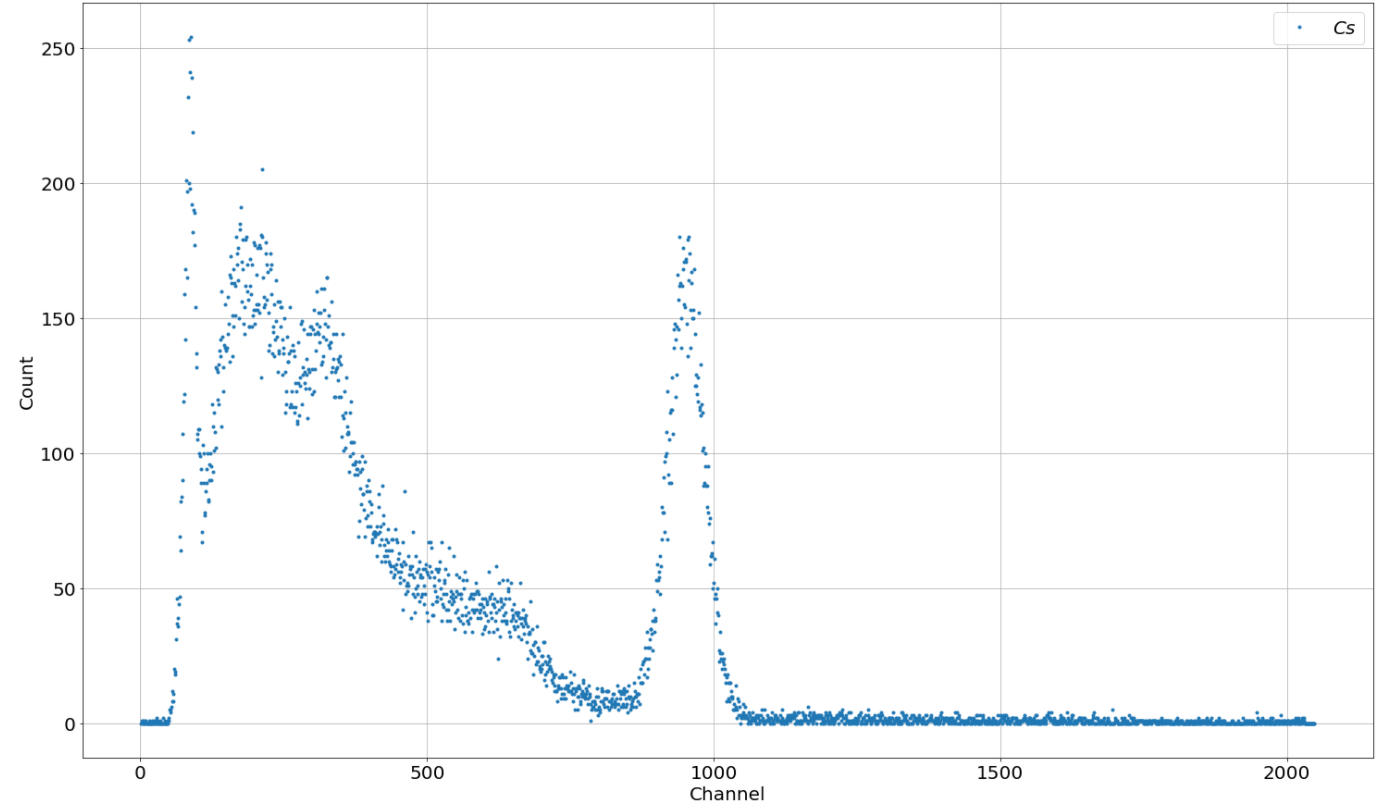
\includegraphics[width=0.8\linewidth]{Cs.png}
  \caption{Спектр ${}^{137}{\text{Cs}}$}
  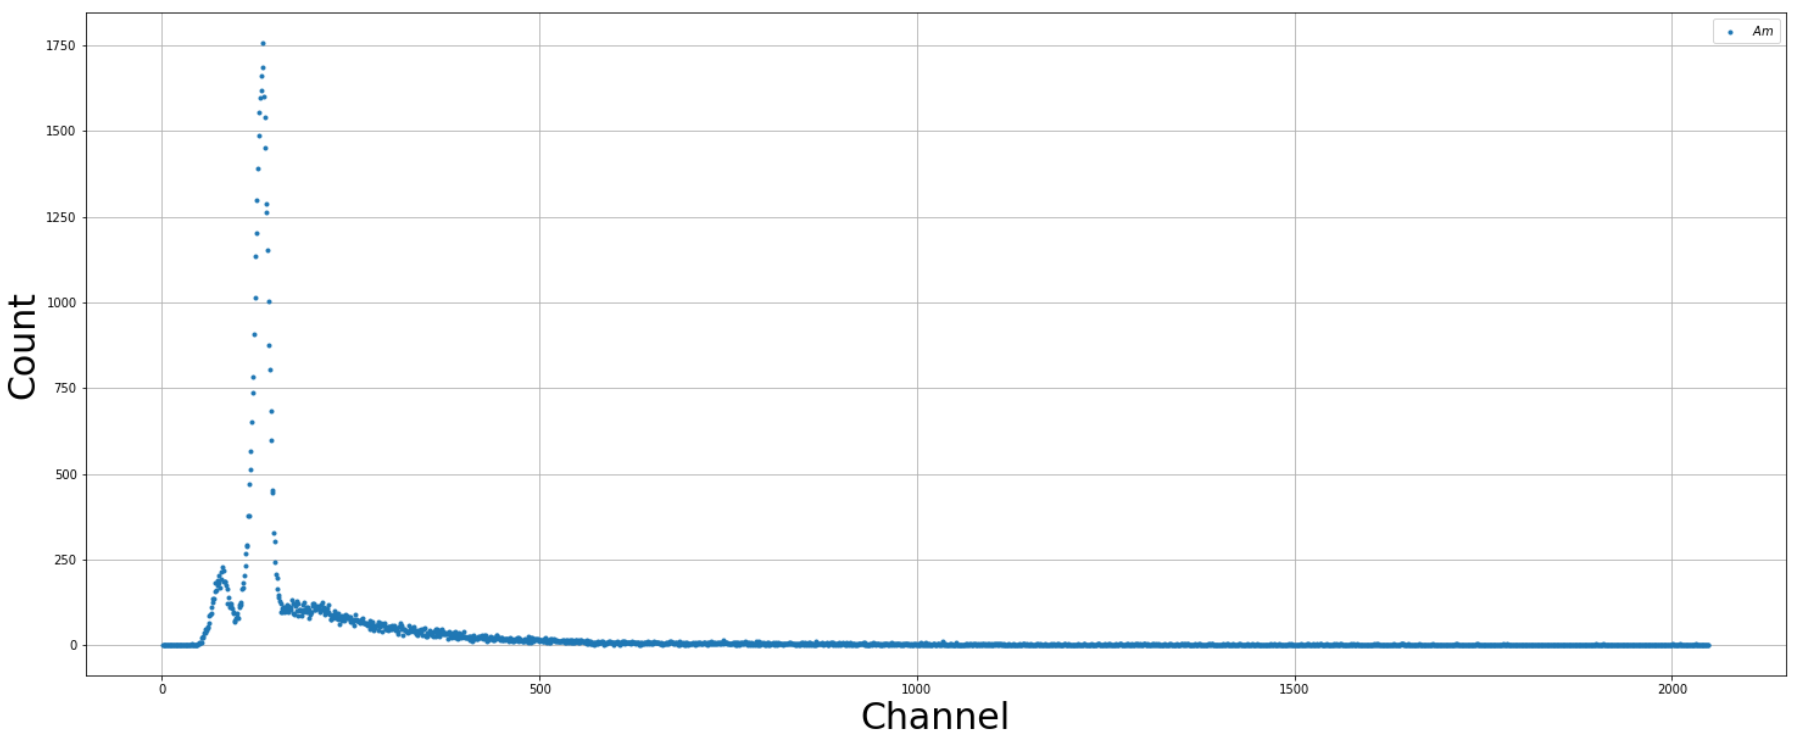
\includegraphics[width=0.8\linewidth]{Am.png}
  \caption{Спектр ${}^{241}{\text{Am}}$}
\end{center}
\end{figure}

\begin{figure}
\begin{center}
  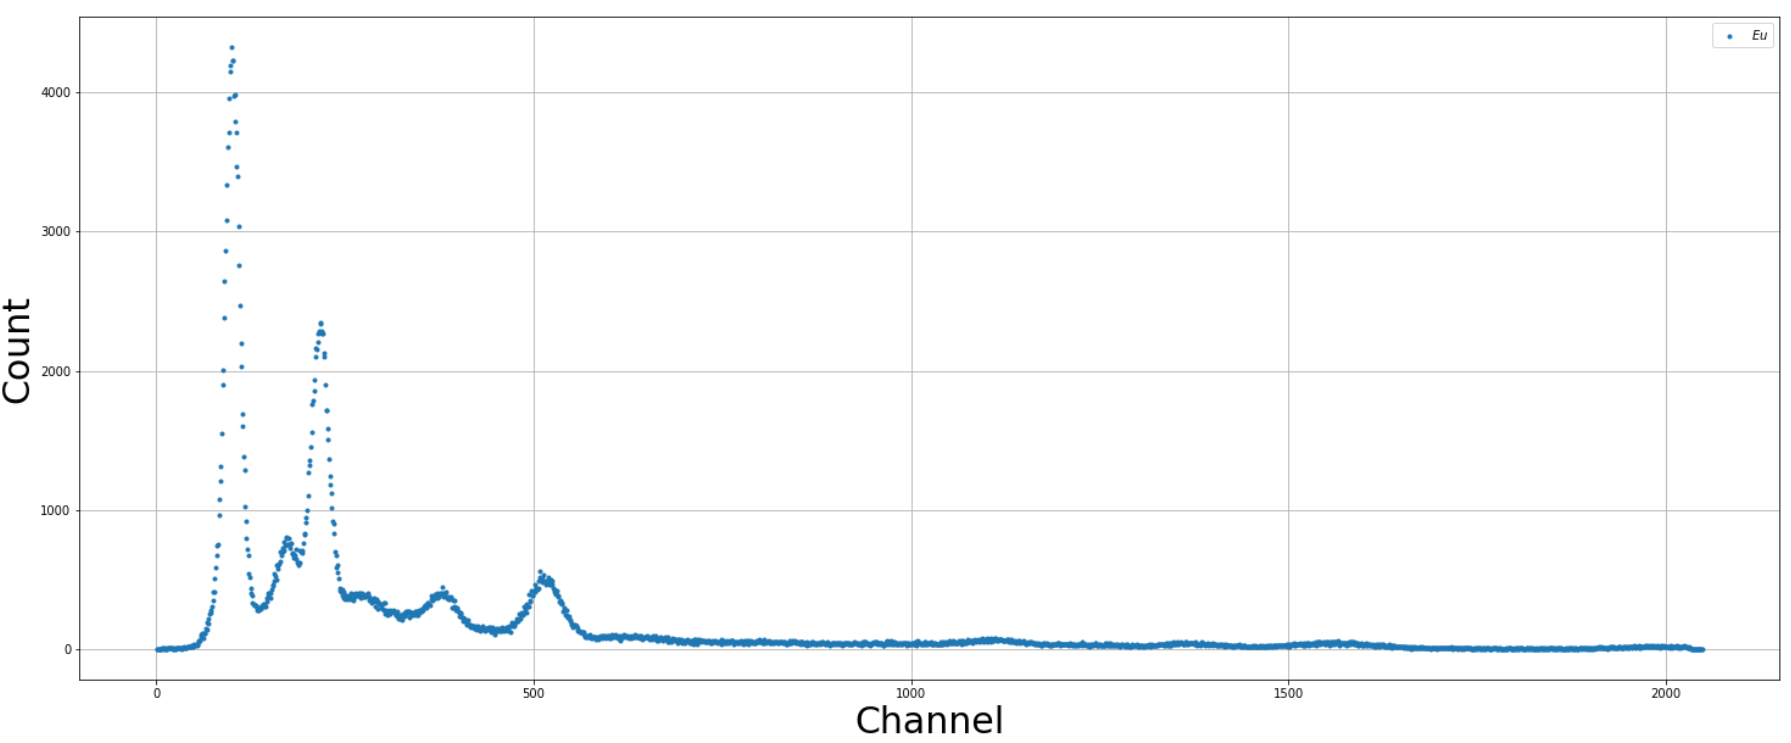
\includegraphics[width=0.8\linewidth]{Eu.png}
  \caption{Спектр ${}^{152}{\text{Eu}}$}
\end{center}
\end{figure}

Используя известные значения пиков в спектрах натрия и цезия, построим
калибровочный график соответствия номера канала определённому значению энергии
(рис. 8).

Получаем уравнение для перехода от номера канала к значению энергии в КэВ:
\begin{center}
    $E = (0.718 \pm 0.004)N_i - (17 \pm 5)$
\end{center}

Используя калибровочный график, определим для всех остальных источников значения
энергии пиков полного поглощения $E_i$ , их ширины на половине высоты $\Delta
E_i$ и энергетическое разрешение $R_i$ . Результаты занесём в таблицу 1. В
последний столбец занесём справочные значения для соответствующих энергий пиков
полного поглощения (знаком (к) отмечены значения, по которым проводилась
калибровка значений прибора)

\begin{table}[h]
\begin{center}
  \caption{Пики полного поглощения различных образцов}
  \label{tab:my_label}
  \begin{tabular}{| c | c | c | c | c | c | c |}
    \hline
    Элемент & $N_i$ & $\triangle N_i$ & $E_i$, МэВ & $\triangle E_i$, МэВ &
    $R_i$ & $E$, МэВ \\
    \hline
    $^{22}$Na & 1811 & 83 & 1.274 & 0.030 & 0.023 & 1.274 (к) \\
    \hline
    $^{60}$Co & 1670 & 37 & 1.171 & 0.027 & 0.023  & 1.173 \\
    \hline
    $^{60}$Co & 1892 & 45 & 1.333 & 0.033 & 0.024 & 1.332 \\
    \hline
    $^{137}$Cs & 967 & 62 & 0.662 & 0.022 & 0.032 & 0.662 (к) \\
    \hline
    $^{241}$Am & 149 & 13 & 0.060 & 0.004 & 0.067 & 0.595 \\
    \hline
    $^{152}$Eu & 235 & 17 & 0.123 & 0.006 & 0.045 & 0.122 \\
    \hline
    $^{152}$Eu & 399 & 31 & 0.243 & 0.010 & 0.040 & 0.245 \\
    \hline
    $^{152}$Eu & 534 & 41 & 0.341 & 0.015 & 0.041 & 0.344 \\
    \hline
  \end{tabular}
\end{center}
\end{table}

По графикам определим энергию характеристического излучения свинца, служащего
защитой спектрометра от внешнего излучения. На всех спектрах, кроме спектра
неизвестного образца, снятого вне установки, в той или иной степени выражена
спектральная линия, соответствующая энергии $75$ КэВ. Эта энергия и есть энергия
характеристического излучения свинца.

Проверим зависимость (6). Для этого построим график зависимости $R^2 = f(1/E)$
(рис. 10). Наблюдается линейная зависимость. Из-за неточностей в определении
полуширины пиков точки не лежат на одной прямой.

Определим энергии края комптоновского поглощения для образцов $^{22}$Na,
$^{137}$Cs, $^{60}$Co, сравним их с соответствующими справочными значениями.

\begin{center}
\begin{table}
\begin{tabular}{| c | c | c |}
  \hline
  Образец & $E_{C_{\text{exp}}}$, МэВ & $E_{C_{\text{th}}}$, МэВ \\
  \hline
  ${}^{60}$Co & $0,922$ & $0.963$ \\
  \hline
  ${}^{137}$Cs & $0,448$ & $0.477$ \\
  \hline
  ${}^{22}$Na & $0,999$ & $1.062$ \\
  \hline
\end{tabular}
\end{table}
\end{center}

В спектрах, где наблюдаются пики обратного рассеяния, определим энергии этих
пиков и сравним измеренные значения с определёнными по формуле (2)

\begin{equation}
  E_{b_s} = \frac{E_{\gamma}}{1 + \frac{2E_{\gamma}}{m_e c^2}}
\end{equation}

\begin{center}
\begin{table}
\begin{tabular}{| c | c | c |}
  \hline
  Образец & $E_{C_{\text{exp}}}$, МэВ & $E_{C_{\text{th}}}$, МэВ \\
  \hline
  ${}^{60}$Co ($E = 1.171$ МэВ) & $0,228$ & $0.209$ \\
  \hline
  ${}^{60}$Co ($E = 1.333$ МэВ) & $0,228$ & $0.214$ \\
  \hline
  ${}^{137}$Cs ($E = 0.662$ МэВ) & $0,198$ & $0.184$ \\
  \hline
\end{tabular}
\end{table}
\end{center}

Эти значения практически совпадают. Пики обратного рассеяния в спектре кобальта,
отвечающие разным пикам полного поглощения, на графике неразрешимы (виден один
широкий пик).
